\subsection{Propuesta de Solucion}
Con base en la problemática presentada, para mejorar el proceso de monitoreo del
kéfir se propone el desarrollo de un Prototipo de un sistema telemático para el
monitoreo de la fermentación artesanal del kéfir mediante sensores y un análisis de
datos. El diseño del sistema busca proporcionar a los productores artesanales de
kéfir una herramienta eficiente que les permita evaluar el estado del kéfir y
determinar si este alcanzo el rango de pH ideal(4.2-4.6) y determinar si la
temperatura durante toda la fermentación se mantuvo de igual manera en el rango
ideal de 18°C a 30°C, mejorando su proceso de producción, reduciendo la
variabilidad en sus resultados al tomar decisiones basadas en datos precisos y
estructurados haciendo comparaciones entre los diferentes parámetros de la
fermentación a través de un historial detallado de fermentaciones previas.
El sistema propuesto se compondrá de cuatro módulos principales como se puede
observar en la \cref{fig:modulos}, cada uno diseñado para abordar un aspecto específico
del proceso de monitoreo de la fermentación.
\begin{figure}[htb]
\centering
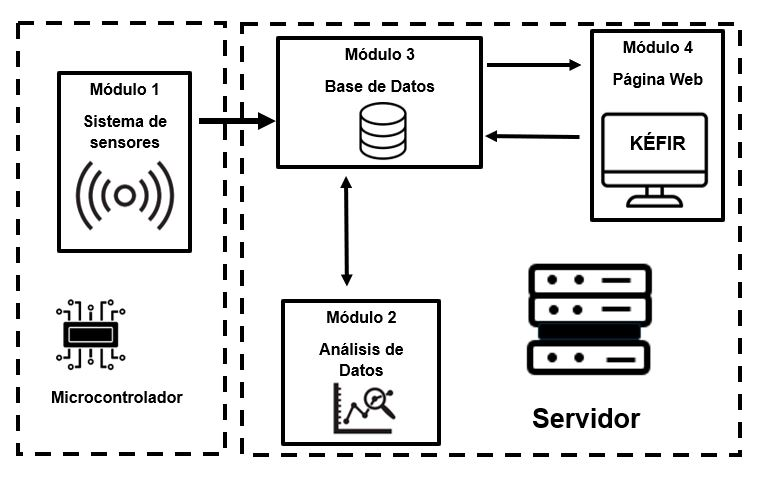
\includegraphics[width=0.7\textwidth]{./Imagenes/Propuesta_Solución/Sistema.JPG}
\caption{Diagrama a Bloques de la interacción de los módulos del sistema}
\label{fig:modulos}
\end{figure} 
A continuación, se describe cada uno de los módulos del sistema:
\subsubsection{Módulo 1:Sistema de Sensores} 
Para el desarrollo de este módulo, se integrarán tres sensores, cuya implementación
dentro del proceso de fermentación es permitida por la NOM-251-SSA1-2009 \cite{zotero-item-56},
siempre y cuando no resulten contaminates para la fermentación.Los sensores se colocarán en la parte interna de la tapa de un frasco
de vidrio hermético, mientras que en la parte superior de dicha tapa se instalará un
microcontrolador, conectado a través de un circuito que enlazará los sensores con
este componente, como se muestra en la \cref{fig:tapa}. Dado que los sensores de
pH y temperatura estarán en contacto directo con el medio de fermentación,
deberán ubicarse cuidadosamente en el interior del frasco, posicionados a una
altura intermedia dentro del líquido. Esta ubicación es crucial, ya que en la parte
superior del kéfir suele formarse una capa de grasa que podría interferir con las
mediciones, mientras que en el fondo se acumulan los búlgaros. Por tanto,
mantenerlos en la zona media del líquido garantiza una lectura representativa y
confiable del proceso de fermentación.
En contraste, el sensor de gas se colocará en el exterior del frasco, conectado
mediante una salida especializada que permitirá la liberación controlada del dióxido
de carbono ($CO_{2}$) generado durante la fermentación. Esta salida evitará la
acumulación de gas dentro del recipiente, lo cual podría generar sobrepresión,
comprometiendo la seguridad del sistema y alterando las condiciones del proceso,
como se muestra en la \cref{fig:frasco}.
\begin{figure}[htb]
\centering
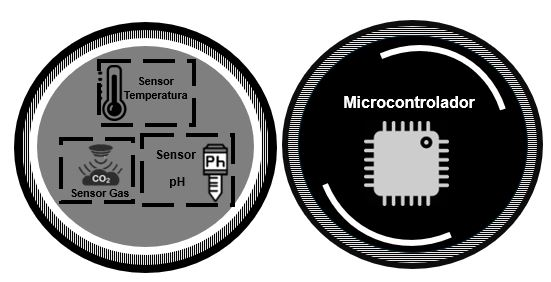
\includegraphics[width=0.5\textwidth]{./Imagenes/Propuesta_Solución/m1_1.JPG}
\caption{Vista Inferior y superior de la tapa del frasco}
\label{fig:tapa}
\end{figure} 
\newline Si bien el prototipo se diseñará inicialmente para un frasco de 1 litro, el sistema
podrá adaptarse a frascos de diferente capacidad, siempre que sean compatibles
con la misma tapa, lo cual garantiza flexibilidad sin comprometer la funcionalidad
del módulo de monitoreo. Dichos sensores se describen a continuación:
\begin{figure}[b!]
\centering
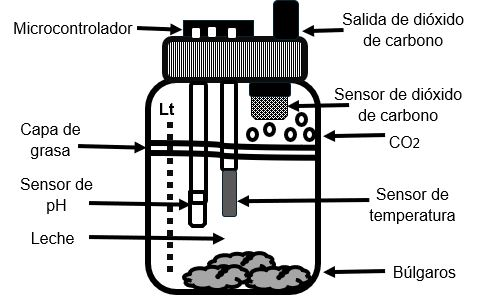
\includegraphics[width=0.5\textwidth]{./Imagenes/Propuesta_Solución/m1_2.JPG}
\caption{Vista completa del frasco}
\label{fig:frasco}
\end{figure} 
\begin{itemize}
    \item \textbf{Sensor de pH:}Censar la disminución gradualmente del pH de la leche
    durante la fermentación y evaluar el pH inicial que este dentro del rango de
    6.6 a 6.8.
     \item \textbf{Sensor de Gas ($CO_{2}$):}Censar la concentración de dióxido de carbono ($CO_{2}$)
    liberado durante la fermentación, lo cual es un indicador adicional de la
    actividad microbiológica y el progreso de la fermentación. Siendo que niveles
    constantes de $CO_{2}$ reflejan una fermentación activa y saludable.
    \item \textbf{Sensor de Temperatura:}Censar la temperatura durante el proceso de la
fermentación y la temperatura inicial de la fermentación.
\end{itemize}

\subsubsection{Módulo 2:Análisis de Datos}
El módulo de análisis de datos se implementará a través de un modelo reglas
basado en un algoritmo de lógica difusa. Su función
será evaluar el estado del proceso de fermentación mediante un modelo de reglas
previamente definidas en las cuales no se requiere una gran cantidad de datos de
parte de los sensores y de la base de datos. Dicho funcionamiento de este módulo
se muestra en la \cref{fig:mod2} y se describe a continuación:
Con base en los datos recolectados por los sensores, el módulo analizará si se ha alcanzado el pH
ideal ubicado entre 4.2 y 4.6, junto con el comportamiento de la temperatura y la
liberación de gas. De esta manera, el sistema no solo verificará si el pH final es
adecuado, sino también si las condiciones de temperatura y producción de gas han
sido consistentes con una fermentación exitosa. En caso contrario, podrá detectar
si, a pesar de que el pH se haya alcanzado, las condiciones de temperatura o de
gas no fueron las adecuadas, lo que indicaría una fermentación no óptima. Además,
si durante el proceso la temperatura se sale del rango ideal, el sistema emitirá
alertas. Todas estas alertas se enviarán a la base de datos para su registro y
visualización en la página web.
\begin{figure}[htb]
\centering
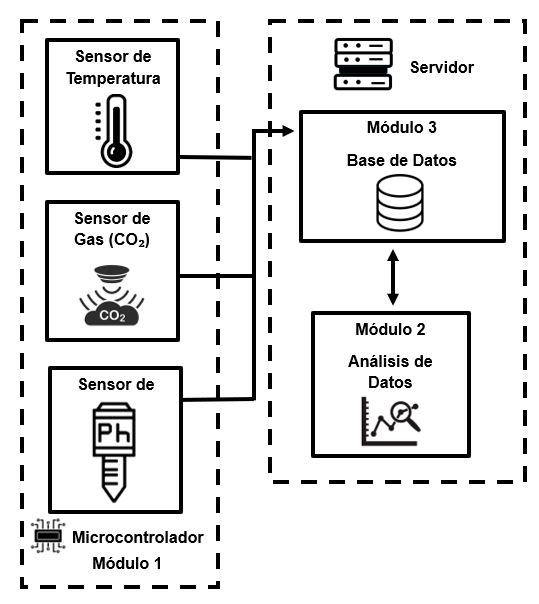
\includegraphics[width=0.5\textwidth]{./Imagenes/Propuesta_Solución/M2.JPG}
\caption{Diagrama a bloques de la integración del módulo 2 con el sistema}
\label{fig:mod2}
\end{figure} 
\subsubsection{Módulo 4:Base de Datos}
Este módulo es crucial para almacenar y gestionar la información relacionada con
las fermentaciones. Sus funciones principales incluyen:
\begin{itemize}
    \item \textbf{Almacenamiento de Datos}Los datos obtenidos por los sensores serán
    almacenados en una base de datos. Además, de las alertas emitidas por el
    análisis de datos.
    \item \textbf{Historial de Fermentaciones}La base de datos mantendrá un historial de
    todas las fermentaciones realizadas por cada productor, lo que permitirá
    realizar un seguimiento detallado de la evolución de cada proceso a lo largo
    del tiempo.
    \item \textbf{Gestión de Usuarios}El sistema almacenará información sobre los
    administradores (productores en jefe) y los productores (usuarios),
    permitiendo una gestión adecuada de los permisos y accesos al sistema
    llevados a cabo en la Página Web.
\end{itemize}
\subsubsection{Módulo 4:Página Web}
La página web es la interfaz de usuario que permitirá a los productores y
administradores interactuar con el sistema. Los usuarios tendrán diferentes niveles
de acceso según su rol, ya sea como productor en jefe (administrador) o como
productores Inicial o Raíz (usuarios). Siendo que estos usuarios tendrán las
siguientes funciones de la página web:
\subsubsection{Productor en jefe (Administrador)}
La interacción de este usuario con el sistema se puede observar en la \cref{fig:admin}, así como se describe a continuación sus principales funciones:
\begin{itemize}
    \item \textbf{Gestión de Usuarios:}El administrador podrá dar de alta o suspender a
    usuarios dentro del sistema, y visualizar la productividad de cada productor
    inicial y raíz así como su relación entre ellos, facilitando la gestión de
    permisos y accesos.
    \item \textbf{Monitoreo de Fermentaciones:}El administrador podrá visualizar el historial
    de fermentaciones de cada productor, así como la fermentación en curso de
    cada uno y recibir alertas si alguna fermentación en curso no está en
    condiciones óptimas. Asimismo, podrá manipular visualmente el historial de
    fermentaciones para poder comparar de manera estadística las
    fermentaciones.
\end{itemize}
\begin{figure}[htb]
\centering
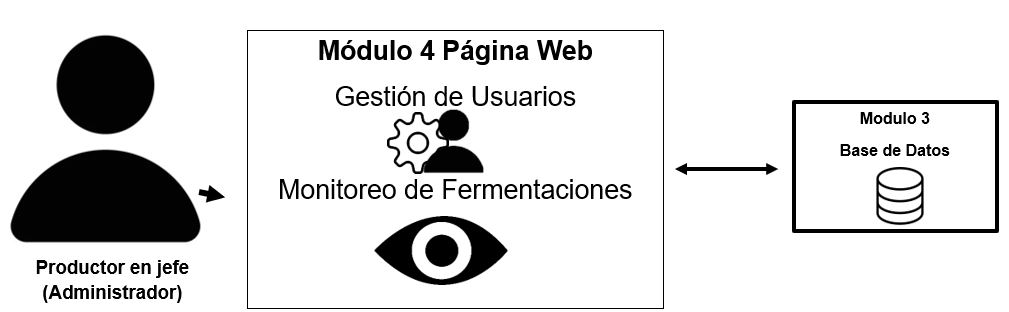
\includegraphics[width=0.5\textwidth]{./Imagenes/Propuesta_Solución/m4_admin.JPG}
\caption{Interacción del Administrador con la Página Web}
\label{fig:admin}
\end{figure} 
El productor tendra dos categorias, productor inicial y productor raiz, mismos que se
describen a continuación:
\subsubsection{Productores Inicial y Raíz (Usuarios)}
\begin{figure}[htb]
\centering
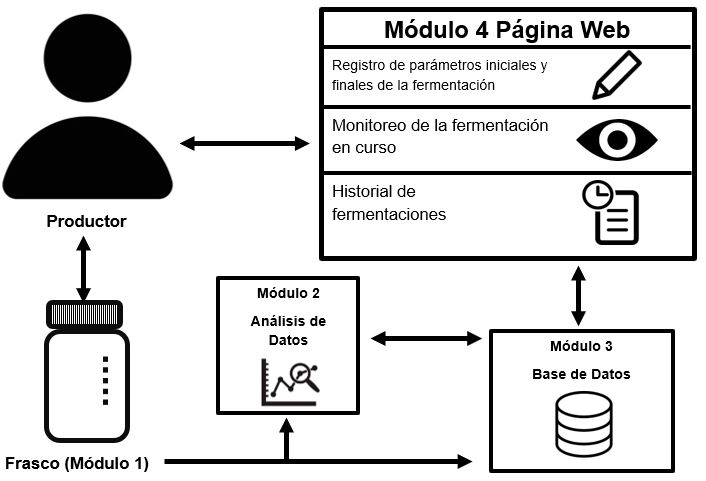
\includegraphics[width=0.5\textwidth]{./Imagenes/Propuesta_Solución/m4_usuario.JPG}
\caption{Interacción del Productor con el sistema}
\label{fig:usuario}
\end{figure} 
El productor, es decir, el usuario registrado en el sistema será responsable de llevar
a cabo el proceso de fermentación del kéfir. Para ello, es indispensable que cada
productor cuente con el frasco descrito en el Módulo 1. La interacción de este
usuario con el sistema se ilustra en la \cref{fig:usuario}, y sus funciones en la plataforma
web se describen a continuación:
\begin{itemize}
    \item \textbf{Registro de parámetros iniciales y finales de la fermentación:}Una vez
que el sistema detecte el inicio de la fermentación en el frasco, se solicitará
al productor que ingrese los datos iniciales: tipo y marca de la leche utilizada,
así como la cantidad de búlgaros empleados. Al finalizar la fermentación, el
productor deberá registrar la cantidad final de búlgaros y proporcionar una
breve descripción del sabor del kéfir obtenido.
    \item \textbf{Monitoreo de la fermentación en curso:}Una vez iniciado el proceso, el
productor podrá visualizar los datos recopilados por los sensores conectados
al frasco de fermentación. Así, como las alarmas emitidas por el módulo 2
(análisis de datos) sobre el estado de la fermentación.
    \item \textbf{Historial de Fermentaciones:}El productor podrá consultar en cualquier
momento su historial de fermentaciones previas, visualizando los registros
completos de cada proceso.
\end{itemize}
\begin{figure}[htb]
\centering
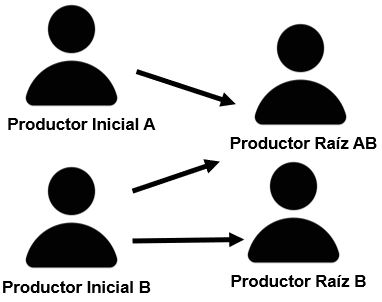
\includegraphics[width=0.5\textwidth]{./Imagenes/Propuesta_Solución/m4_usuarios.JPG}
\caption{Relación usuarios raíz con su origen}
\label{fig:raiz}
\end{figure} 
Mientras que el prodcutor raíz será otra categoría la cual contará con las mismas funciones que el
productor inicial; sin embargo, se considerará un usuario derivado de uno o más
productores como se ejemplifica en la \cref{fig:raiz}, ya que en el proceso de
fermentación del kéfir los búlgaros se reproducen y pueden ser compartidos con
otros productores. De esta forma, el nuevo usuario hereda los cultivos del productor
original, pero se considera independiente, ya que sus parámetros de fermentación
como el tipo de leche, la temperatura o el tiempo pueden diferir. Esta relación entre
usuarios permite trazar el origen de los búlgaros y analizar su trayectoria, lo cual
puede ser útil para los productores al conocer el linaje o procedencia de sus cultivos.
\subsection{Objetivo}
Diseñar e implementar un prototipo de un sistema telemática de monitoreo no
invasivo para la fermentación de kéfir artesanal de leche de vaca, mediante la 
recopilación, análisis y visualización de los datos obtenidos por parte de los
sensores.
\subsection{Objeivos específicos}
\begin{enumerate}
    \item Seleccionar e integrar un microcontrolador y sensores no invasivos de
            temperatura, pH y $CO_{2}$ mediante un circuito que permita su conexión y el
            envío de datos hacia la base de datos.
    \item  Desarrollar una interfaz web enfocada a cada usuario (administrador,
            productor inicial y raíz), que permita la visualización de los datos recopilados
            por los sensores y del análisis de datos, así como de las alarmas generadas
            por el sistema.
    \item Diseñar e implementar un modelo de reglas basado en criterios definidos que
            interprete los datos de los sensores y evalúe el estado de la fermentación,
            verificando que el pH alcance el rango ideal (4.2 a 4.6) y que la temperatura
            se mantenga dentro del intervalo óptimo durante todo el proceso.
    \item Analizar, estructurar e implementar una base de datos que permita almacenar
            los datos del monitoreo, así como las alarmas emitidas por el sistema, y
            gestionar la autenticación de los usuarios de la página web
    \item Realizar pruebas de fermentación con distintos parámetros iniciales para
            validar el funcionamiento del sistema.
\end{enumerate}

\subsection{Alcances}
\begin{enumerate}
    \item El sistema va dirigido únicamente a pequeños y medianos productores de
        kéfir artesanal elaborado con leche de vaca de origen comercial que cumplan
        con la Norma Oficial Mexicana NMX-F-446-1984, ubicados en la ciudad de
        México que requieran tener un mejor monitoreo en los parámetros de sus
        fermentaciones, los cuales deberán contar con una computadora para
        acceder al sistema.
    \item Dado que es un prototipo, el sistema se enfocará únicamente en la
        visualización de los datos recolectados por los sensores e interpretados por
        el análisis de datos a través de la página web con el único fin de monitorear.
        El sistema no contara con funciones de manipulación o control de los
        parámetros en los sensores ni del módulo 2(análisis de datos).
    \item El sistema estará limitado a un frasco por usuario (productor), con el fin de
        facilitar un monitoreo más preciso y controlado durante las pruebas del
        prototipo. Asimismo, el sistema solo permitirá una sesión activa por usuario,
        evitando la duplicación de datos o posibles inconsistencias.
    \item Se establecerán los parámetros específicos que debe cumplir el proceso de
        fermentación, con base en normativas técnicas y condiciones óptimas del
        kéfir, los cuales serán utilizados por el análisis de datos para evaluar el
        proceso y emitir alertas si es necesario.
    \item Debido a la sensibilidad y variabilidad que pueden presentar los sensores,
        deberán calibrarse y limpiarse manualmente después de cada proceso de
        fermentación, para esto se le incorporará al sistema una función de prueba
        para realizar dicha calibración, esto con el fin de tener una mejor medición
        por parte de los sensores.
\end{enumerate}

\subsection{Justificación}

Debido a la alta variabilidad inherente en los procesos de producción artesanal 
del kéfir influida por la diversidad y evolución de las cepas microbianas en los granos 
(búlgaros), muchos sistemas de monitoreo actuales resultan limitados, ya que suelen basarse en 
una sola cepa estandarizada o se restringen a parámetros fijos como pH y temperatura, 
sin considerar la producción de CO$_2$ como indicador directo de la actividad metabólica y 
vitalidad microbiana. Además, estos sistemas a menudo asumen que los productores poseen un alto 
nivel de \textit{expertise} técnico, tratándolos como expertos capaces de interpretar datos crudos 
y complejos en entornos de producción altamente variables y poco estructurados.

De aquí surge la importancia del desarrollo de este sistema telemático no invasivo, 
que incorpora de manera integral el monitoreo en tiempo real de pH, temperatura y CO$_2$. 
A diferencia de enfoques convencionales que ignoran o subestiman el CO$_2$ un subproducto 
clave generado por la actividad levadurienta y bacteriana durante la fermentación heteroláctica, 
este prototipo permite evaluar con precisión aspectos críticos como la mayor o menor actividad 
de una cepa respecto a otra, la viabilidad y el envejecimiento de los granos 
(dado su tiempo de vida limitado), o incluso riesgos asociados a un exceso de CO$_2$ que podría comprometer
 la evolución del proceso o la seguridad del recipiente.

Además, al registrar el árbol genealógico de las cepas utilizadas 
(origen, evolución y características a lo largo de producciones sucesivas),
 el sistema ofrece un registro estructurado y trazable, clave en la elaboración artesanal 
 mexicana donde las cepas locales presentan variabilidad natural y potencial no explorado. 
 Esto no solo facilita la identificación de cepas más útiles o adaptadas al contexto nacional, 
 sino que también habilita estudios científicos sobre la diversidad microbiana del kéfir en México, 
 contribuyendo al conocimiento de probióticos locales.

Gracias al procesamiento mediante reglas de lógica difusa que modela la incertidumbre 
y variabilidad natural del proceso, el sistema transforma datos complejos en visualizaciones 
amigables y comprensibles, permitiendo que productores sin formación técnica especializada 
interpreten fácilmente el estado de la fermentación. De esta forma, convierte un proceso
 inherentemente elaborado y dinámico en algo accesible y práctico, facilitando decisiones informadas
  en tiempo real sin requerir \textit{expertise} avanzado.

No obstante, este sistema se enfoca primordialmente en el monitoreo base 
fundamental de cualquier optimización productiva, ya que un análisis detallado y
 basado en datos puede sentar las bases para futuros sistemas de control automatizado más específicos.

En conclusión, el diseño único de este prototipo telemático es económico, accesible, 
sin requerir infraestructura previa y adaptado a la realidad de pequeños productores 
artesanales representa un avance significativo al transitar de procesos empíricos a uno 
más estructurado y basado en evidencia. Al reducir mermas entre producciones, mejorar la 
consistencia y calidad del producto final, democratizar el acceso a información técnica mediante
 interfaces amigables y ampliar el panorama sobre la salud y utilidad de las cepas mexicanas, 
 contribuye de forma efectiva a fortalecer y profesionalizar la elaboración artesanal del kéfir, 
 potenciando su valor como alimento funcional sostenible en el contexto nacional.

 \subsection{Metodología}
El presente proyecto se centra en el desarrollo de un prototipo de sistema telemático destinado
al monitoreo de la fermentación artesanal del kéfir de leche. Para garantizar 
su correcta implementación, resulta fundamental contar con una metodología 
estructurada que permita abordar cada una de las etapas del proyecto de manera ordenada, 
sistemática y eficiente. De esta manera, no solo se asegura el cumplimiento de los objetivos 
establecidos, sino que además se incorporan los antecedentes teóricos y técnicos indispensables 
para validar y justificar tanto el diseño conceptual como la posterior implementación del sistema.
Con base en lo anterior, se propone la siguiente metodología dividida en cinco etapas principales:

\subsubsection{Revisión Bibliográfica}

En la etapa de revisión bibliográfica, se realizó un análisis exhaustivo a través del estado del arte,
sobre el proceso de fermentación artesanal del kéfir de leche, incluyendo los parámetros clave 
que determinan su calidad (como temperatura, pH y evolución de acidez)así como investigaciones
previas que han destacado brechas significativas en el monitoreo de este proceso.
Entre estas brechas se identificó la escasez de soluciones accesibles y adaptadas específicamente 
al kéfir artesanal en contextos locales, como la Ciudad de México, donde los productores 
suelen depender de métodos empíricos sin soporte tecnológico estructurado, lo que permitió 
justificar la necesidad del prototipo propuesto.

Además, se estudiaron 
sistemas telemáticos de monitoreo en procesos fermentativos similares, tecnologías de sensores 
de bajo costo, aplicaciones de lógica difusa en evaluación de procesos biológicos y plataformas 
para almacenamiento y visualización de datos . 
Esta revisión permitió establecer un marco teórico sólido que orienta el diseño y 
desarrollo del prototipo, identificando las mejores prácticas y tecnologías compatibles.

\subsubsection{Análisis de la solución}

En la etapa de análisis de la solución, se llevaron a cabo los requerimientos
funcionales y no funcionales del sistema de cada módulo. Se evaluaron y seleccionaron los 
componentes necesarios en hardware (sensores de temperatura y pH,así como microcontroladores 
y protocolo de comunicación) y software para cada módulo .
No obstante se consideraron aspectos básicos en la selección de componentes como compatibilidad 
entre módulos, bajo consumo energético y costos.Permitiendo garantizar 
una solución eficiente, escalable y adaptada a las condiciones para desarrollar el proyecto
para producción artesanal 
en la Ciudad de México, maximizando así el rendimiento y la viabilidad del prototipo.

 \subsubsection{Diseño del sistema}

En la etapa de diseño del sistema, se definió la estructura modular del prototipo con base en
el análisis previo y los objetivos establecidos del proyecto. Se desarrollaron los diagramas 
de arquitectura general del sistema, detallando la interacción entre los cuatro módulos principales.

Por lo que respecta al módulo de sensores, se diseñaron los esquemas de conexión del hardware,
incluyendo la disposición física de los sensores en el frasco de fermentación y su enlace con
el microcontrolador. Para el módulo de análisis de datos, se definieron los dominios difusos y las reglas
necesarias para evaluar el estado de la fermentación basándose en los datos recopilados por
los sensores. En cuanto al módulo de base de datos, se estructuró el esquema de la base de datos
para almacenar de manera eficiente los datos de fermentación y las alertas generadas. Finalmente,
se diseñó la interfaz de usuario de la página web, asegurando una experiencia intuitiva y
accesible para los diferentes tipos de usuarios (administradores y productores).

\subsubsection{Implementación del prototipo}
Para la etapa de implementación del prototipo, se procedera a ensamblar físicamente los componentes
del sistema según el diseño establecido. Esto incluyó la integración de los sensores de pH,
temperatura y CO$_2$ con el microcontrolador, así como la configuración del circuito necesario para su funcionamiento.
Asimismo, se desarrollara el módelo de logica difusa para el análisis de datos, programando las reglas y dominios
definidos en la etapa de diseño. Paralelamente, se implementará la base de datos, creando las tablas y relaciones necesarias para almacenar la información de fermentación.
Finalmente, se desarrollará la página web, implementando las funcionalidades y la interfaz de usuario diseñada previamente.

\subsubsection{Pruebas y validación}
En la etapa de pruebas y validación, se llevarán a cabo una serie de ensayos para evaluar el funcionamiento
integral del prototipo.
Posteriormente a la implementación, se realizarán pruebas unitarias en cada módulo para verificar su correcto desempeño individual.
Una vez validados los módulos por separado, se procederá a realizar pruebas de integración para asegurar
que todos los componentes del sistema funcionen de manera conjunta y coordinada.
Por consiguiente, se evaluaran los objetivos establecidos por medio del funcionamiento del sistema para corroborar 
si es capaz de monitorear adecuadamente el proceso de fermentación del kéfir con diferentes parámetros iniciales y diferentes cepas de búlgaros.
Docuementando los resultados obtenidos y realizando ajustes necesarios para optimizar el rendimiento del prototipo.




